\documentclass[12pt]{article} % Клас документа, шрифт 12pt

\usepackage[utf8]{inputenc} % UTF-8 кодування
\usepackage[T2A]{fontenc} % Шрифти кирилиці
\usepackage[ukrainian]{babel} % Українська мова
\usepackage{geometry} % Поля сторінки
\geometry{a4paper, margin=2cm} % Формат A4, поля 2 см

\usepackage{xcolor} % Кольори
\usepackage{tcolorbox} % Кольорові рамки
\usepackage{graphicx} % Зображення
\usepackage{amsmath, amsthm, amssymb} % Математика, теореми, символи

\usepackage{caption} % Підписи до рисунків
\captionsetup{labelsep=period} % Роздільник у підписах "Рис. 1."

\newtheorem{theorem}{Теорема} % Середовище для теорем

\usepackage{fancyhdr} % Колонтитули
\pagestyle{fancy} % Використання fancyhdr
\fancyhf{} % Очищення стандартних колонтитулів
\setlength{\headheight}{15pt} % Висота верхнього колонтитулу

\newcommand{\student}{Гуцол Альона} % ПІБ студента
\newcommand{\labdate}{\today} % Дата

\fancyhead[L]{\student} % Лівий верхній колонтитул
\fancyhead[R]{\labdate} % Правий верхній колонтитул
\fancyfoot[C]{\thepage} % Нижній колонтитул — номер сторінки

\begin{document}

\begin{center}
    \Large \textbf{Лабораторна робота № 9} \\
    \large \textbf{Тема: Набір математичних текстів та автоматизація в LaTeX}
\end{center}

\section*{Мета роботи}
\textit{навчитися вводити математичні формули та структурувати документ, використовувати кольорові рамки для визначень, теорем та прикладів, а також вставляти зображення}.

\section{Короткі теоретичні відомості}

\begin{tcolorbox}[colback=blue!10!white, colframe=blue!80!black, title=Визначення]
Квадратом називають прямокутник, у якого всі сторони рівні.
\end{tcolorbox}

На рисунку \ref{fig:kvadrat} зображено квадрат $ABCD$. Прямокутник є паралелограмом, тому і квадрат --- паралелограм, у якого всі сторони рівні, тобто він є і ромбом. Отже, квадрат має властивості прямокутника та ромба. 

\begin{figure}[h]
    \centering
    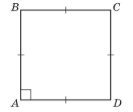
\includegraphics[width=0.20\textwidth]{foto1.png}
    \caption{Квадрат $ABCD$}
    \label{fig:kvadrat}
\end{figure}

\medskip
\textit{Властивості квадрата:}
\begin{enumerate}
    \item Усі кути квадрата прямі.
   \item Периметр $P_{ABCD}=4AB$.
\item Діагоналі квадрата між собою рівні (рис. \ref{fig:diag}).
\item Діагоналі квадрата взаємно перпендикулярні і точкою перетину діляться навпіл (рис. \ref{fig:diag}).
\item Діагоналі квадрата ділять його кути навпіл, тобто утворюють кути $45^\circ$.
\item Точка перетину діагоналей квадрата рівновіддалена від усіх вершин: $AO = BO = CO = DO$.
\end{enumerate}

\begin{figure}[h]
    \centering
    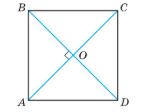
\includegraphics[width=0.20\textwidth]{foto2.png}
    \caption{Діагоналі квадрата}
    \label{fig:diag}
\end{figure}

\begin{tcolorbox}[colback=green!5!white, colframe=green!75!black, title=Приклад 1]
Точки $K$ і $M$ належать відповідно діагоналям $BD$ і $AC$ квадрата $ABCD$, причому $AM=\frac14 AC$, $BK=\frac14 BD$. Доведіть, що $\triangle ADM = \triangle BAK$(рис. \ref{fig:prykl}).
\end{tcolorbox}

\begin{figure}[h]
    \centering
    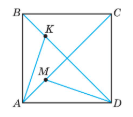
\includegraphics[width=0.20\textwidth]{foto3.png}
    \caption{Ілюстрація до прикладу}
    \label{fig:prykl}
\end{figure}

\begin{proof}
\begin{enumerate}
    \item $\angle MAD = \angle ABK = 45^\circ$, а $AD = AB$ як сторони квадрата.
  \item Оскільки $AC = BD$ як діагоналі квадрата і $AM=\frac14 AC$, $BK=\frac14 BD$, то $AM=BK$.
\item Отже, $\triangle ADM = \triangle BAK$ за двома сторонами і кутом між ними.
\end{enumerate}
\end{proof}

\section{Ознаки квадрата}

\begin{tcolorbox}[colback=blue!5!white, colframe=blue!75!black, title=Ознаки квадрата]
\begin{theorem}
\begin{enumerate}
    \item Якщо діагоналі прямокутника взаємно перпендикулярні, то він є квадратом.
    \item Якщо діагоналі ромба між собою рівні, то він є квадратом.
\end{enumerate}
\end{theorem}
\end{tcolorbox}

\begin{proof}
1) Прямокутник є паралелограмом, а паралелограм із взаємно перпендикулярними діагоналями є ромбом. Отже, у даного прямокутника всі сторони рівні, тому він є квадратом.
2) Ромб є паралелограмом, а паралелограм з рівними діагоналями є прямокутником. Отже, у даного ромба всі кути прямі, тому він є квадратом.
\end{proof}

\section*{Контрольні запитання}
\begin{enumerate}
    \item Що таке квадрат? Які його властивості?
    \item Які ознаки квадрата через діагоналі?
    \item Як вставляти зображення та підпис у LaTeX?
    \item Як оформити визначення, теорему та приклад у кольоровій рамці?
\end{enumerate}

\end{document}